\section{Introduction}

\subsection{Motivation}

Roughly one in six people worldwide lives with a significant disability. For many of them an
assistive device is the primary way for them to perceive and interact with the world.
Accessibility is the practice of designing hardware and software so that people with
temporary or permanent physical, sensory, or cognitive differences have an equal opportunity to use them. Unavailibility of accessible features exclude a portion of the population from conveniences of electronic, which we might argue that they are effectively isolated from communication. Building inclusively is therefore both an act of basic
fairness and, increasingly, a legal obligation.

This report documents our group research on existing norms and regulation around the inclusiveness that applications should implements, as well as how our group apply them to a podcast and audiobook player to be usable by people who rely on assistive technology such as the TalkBack screen reader, Switch Access, and large display fonts. We chose an
audio-first product as listening to audio content is one of the few digital experiences that a user with vision problems can enjoy on completely equal terms with a normal vision user,

\subsection{Project goal and scope}

Our goal was to take a typical, non-inclusive to vision-impaired people UI and improve it into an accessible one, then explain and justify every technique we applied. The deliverable is a front-end only Jetpack Compose application (all data is mocked behind a repository interface, with no real backend) along with this report, which is organised around four contributions:

\begin{itemize}[leftmargin=1.4em]
	\item \textbf{Background} : the legal and technical foundations of Android accessibility.
	\item \textbf{Core semantics} : labelling, roles, state, touch targets, and font scaling.
	\item \textbf{Advanced semantics} : merging, traversal order, and custom screen-reader actions.
	\item \textbf{Testing and evaluation} : how we verify the result and honestly assess trade-offs.
\end{itemize}

\subsection{What ``done'' looks like}

Throughout the project we held ourselves to a simple bar: a person who never looks at the
screen should be able to open the app, browse shows, pick an episode, and control playback using
TalkBack alone. Figure~\ref{fig:appflow} shows the three-screen user flow that a sighted user sees;
the rest of the report explains what a screen-reader user hears and does at each step.

\begin{figure}[h]
	\centering
	\begin{subfigure}{0.31\textwidth}
		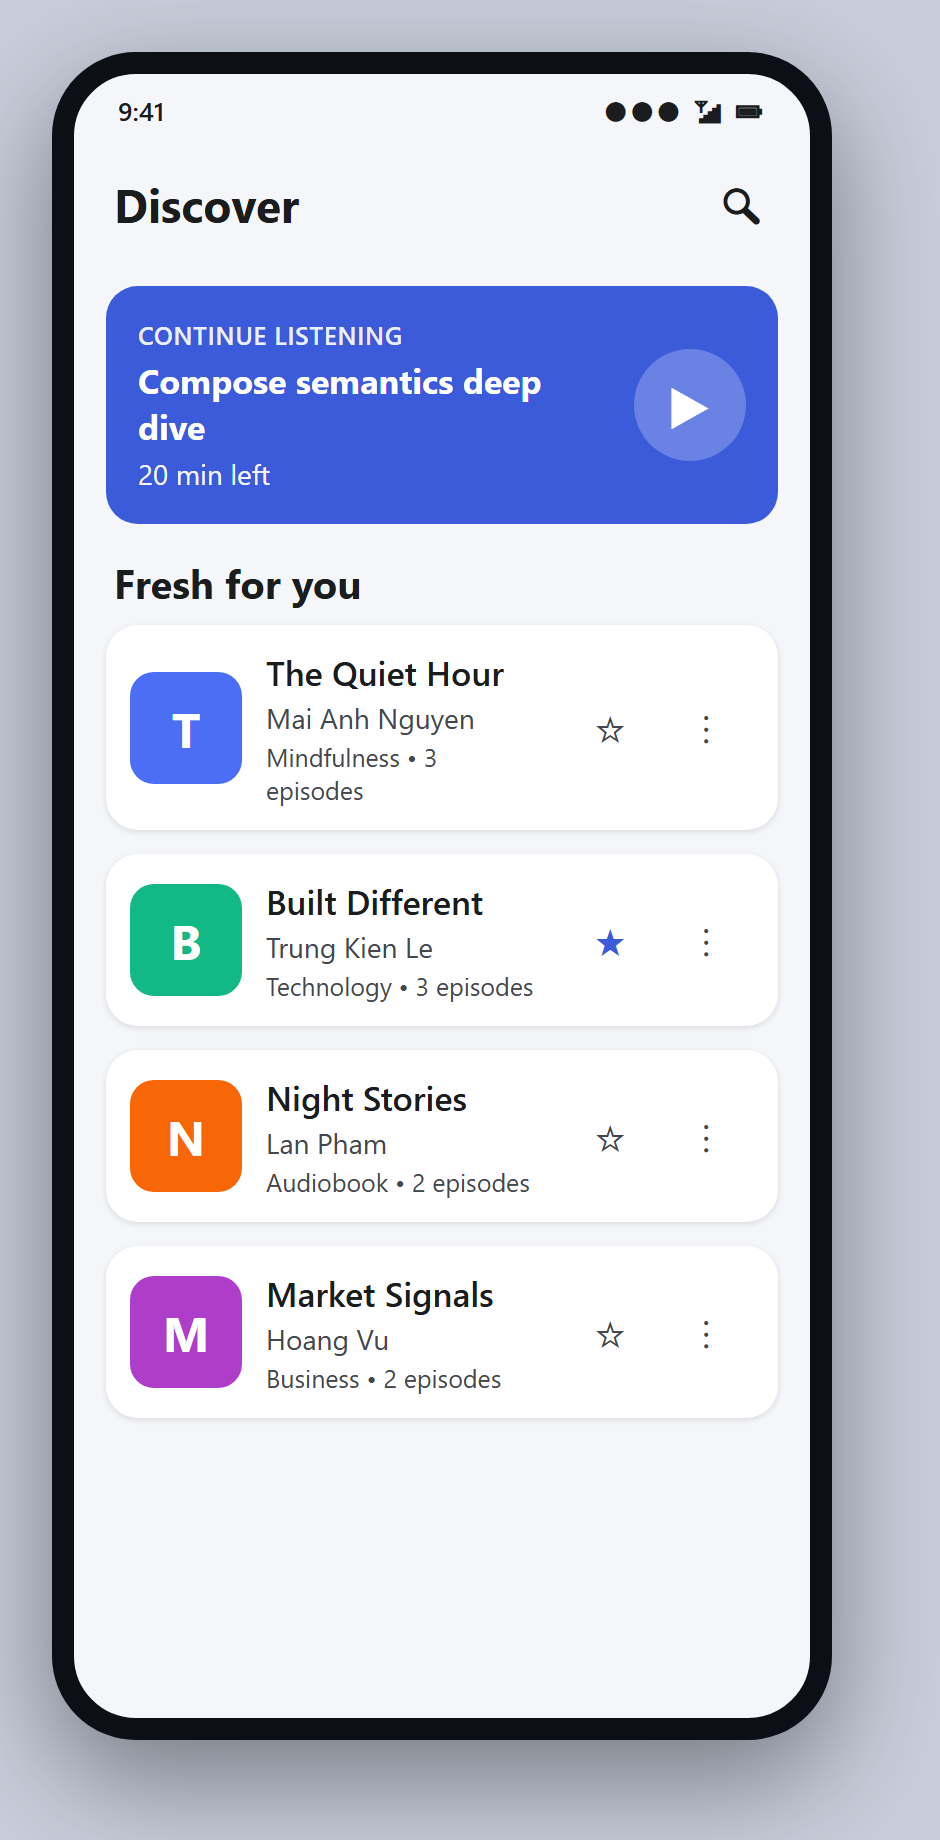
\includegraphics[width=\linewidth]{images/home.png}
		\caption{Discover}
	\end{subfigure}\hfill
	\begin{subfigure}{0.31\textwidth}
		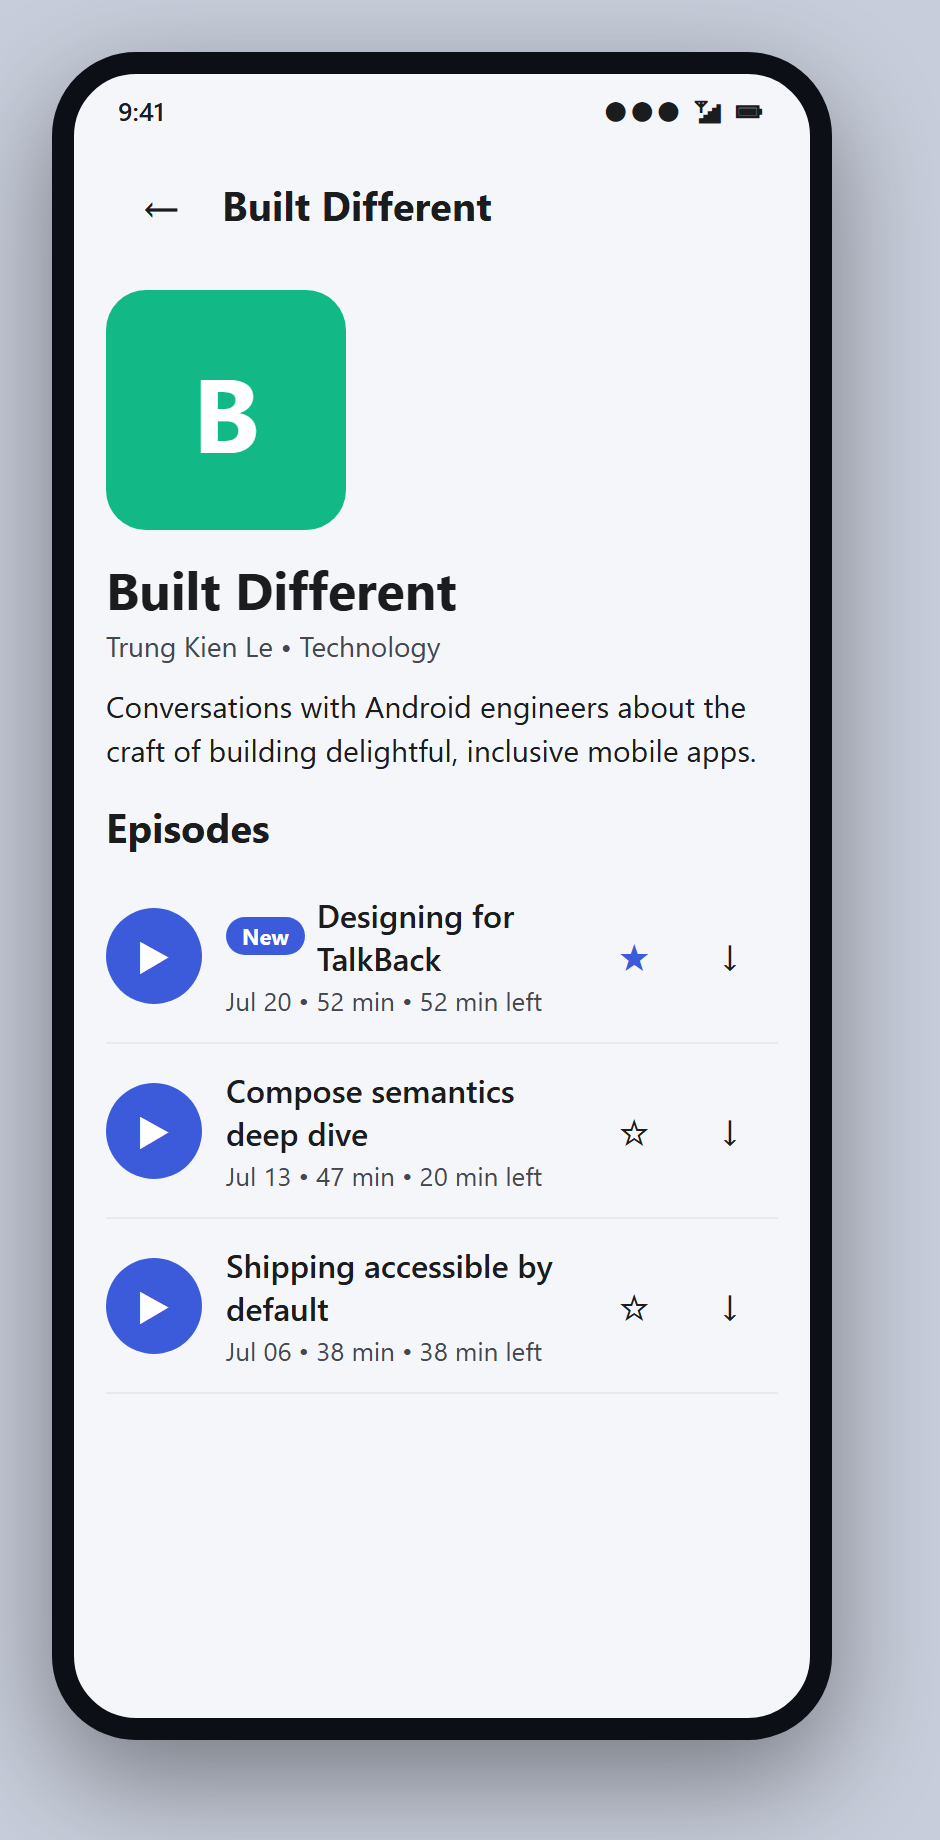
\includegraphics[width=\linewidth]{images/detail.png}
		\caption{Podcast detail}
	\end{subfigure}\hfill
	\begin{subfigure}{0.31\textwidth}
		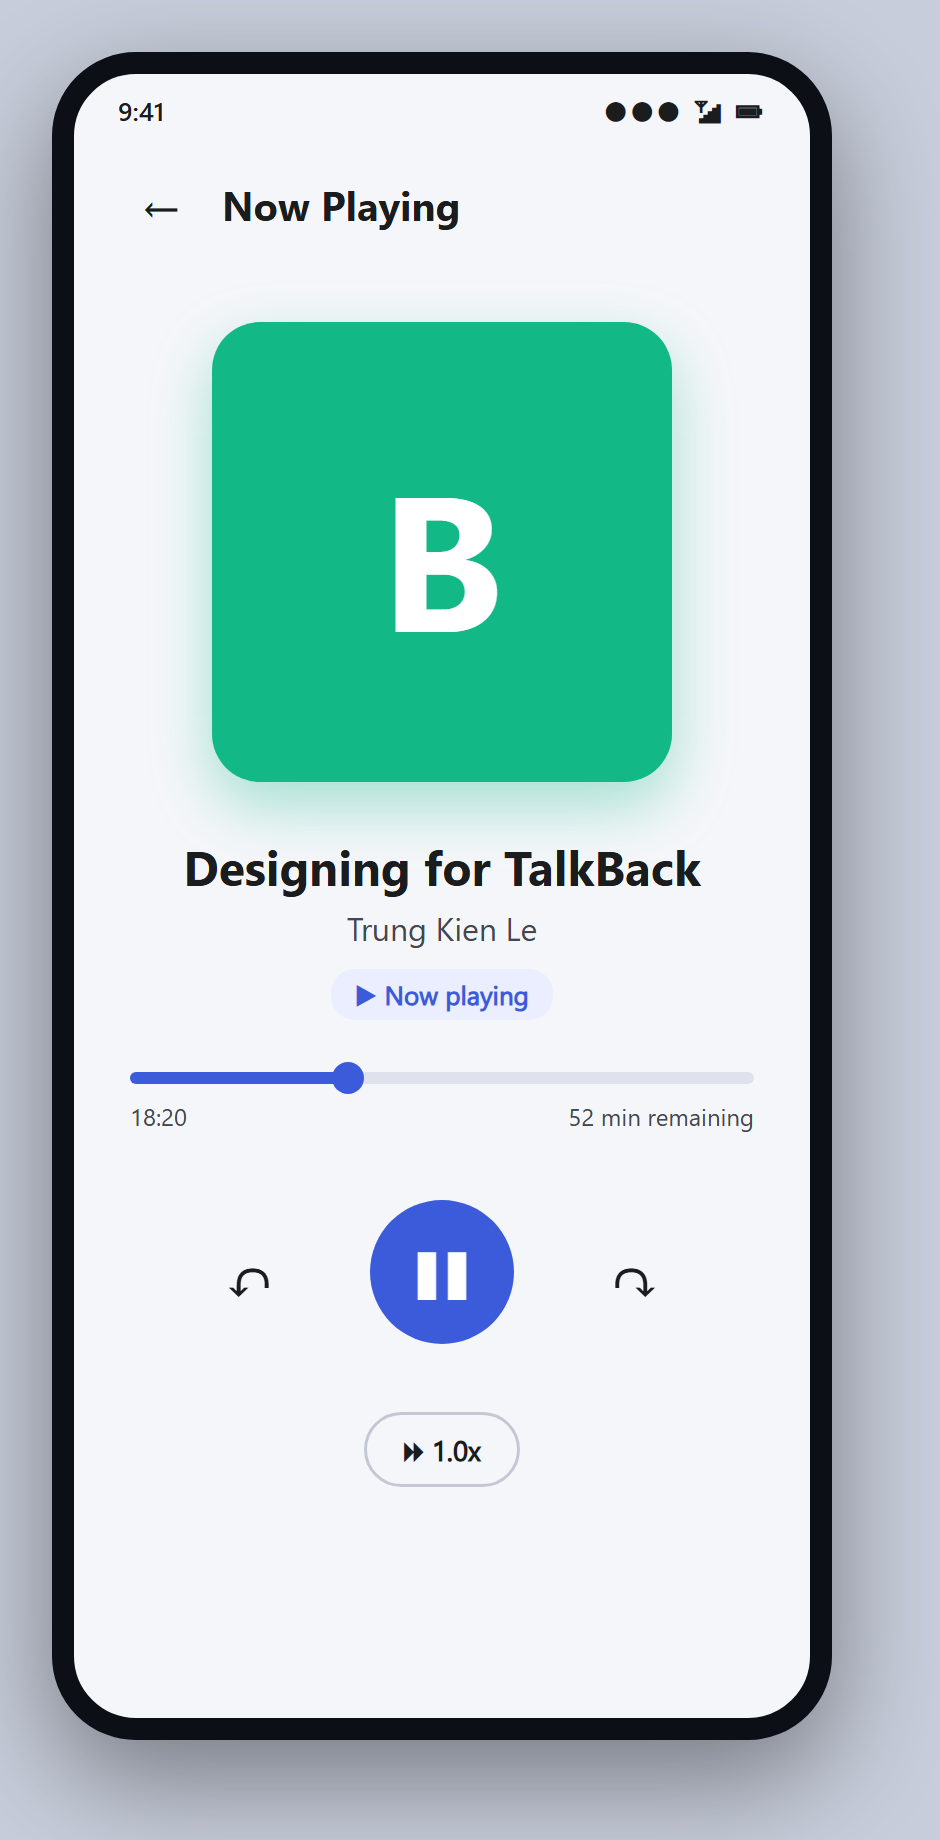
\includegraphics[width=\linewidth]{images/player.png}
		\caption{Now Playing}
	\end{subfigure}
	\caption{The three screens of the case-study app. The user flow is
		\textbf{Discover $\rightarrow$ Podcast detail $\rightarrow$ Now Playing}, with a
		``Continue listening'' shortcut on the home screen.}
	\label{fig:appflow}
\end{figure}
